\chapter{Appendix for part I}
\label{chap-app-pomdp}
\section{Reproducig Topin et. al. 2021}

\begin{table}
    \centering
    \caption{IBMDP hyperparameters. We try 12 different IBMDPs. In green we highlight the hyperparameters from the original paper and in red we highlight the hyperparameter names for which author do not give information.}\label{tab:ibmdp-params}
    \begin{tabular}{ll}
    \toprule
    \textbf{Hyperparameter} & \textbf{Values}\\
    \midrule
    Discount factor $\gamma$ & \textcolor{green}{1} \\
    Information gathering actions parameter $q$ & 2, \textcolor{green}{3} \\
    Information gathering actions rewards $\zeta$ & \textcolor{green}{-0.01}, 0.01 \\
    \textcolor{red}{Depth control} & Done signal, negative reward, none \\ 
    \bottomrule
    \end{tabular}
    \end{table}

\begin{table}
    \centering
    \caption{(Modified) DQN trained on $10^6$ timesteps. This gives four different instantiation of (modified) DQN. Hyperparameters not mentioned are stable-baselines3 default. In green we highlight the hyperparameters from the original paper and in red we highlight the hyperparameter names for which author do not give information.}\label{tab:ibmdp-rl1}
    \begin{tabular}{ll}
    \toprule
    \textbf{Hyperparameter} & \textbf{Values}\\
    \midrule
    Buffer size & \textcolor{green}{$10^6$} \\
    Random transitions before learning & \textcolor{green}{$10^5$} \\
    Epsilon stard & 0.9, \textcolor{green}{0.5} \\
    Epsilon end & \textcolor{green}{0.05} \\
    Exploration fraction & \textcolor{green}{0.1} \\
    Optimizer & \textcolor{green}{RMSprop ($\alpha = 0.95$)}\\
    Learning rate & \textcolor{green}{$2.5\times10^{-4}$}\\
    Networks architectures & \textcolor{green}{[128, 128]}\\
    \textcolor{red}{Networks activation} & $\operatorname{tanh()}$, $\operatorname{relu()}$\\
    \bottomrule
    \end{tabular}
    \end{table}

\begin{table}
    \centering
    \caption{(Modified) PPO trained on $4\times10^6$ timesteps. This gives two different instantiation of (modified) PPO. Hyperparameters not mentioned are stable-baselines3 default. In green we highlight the hyperparameters from the original paper and in red we highlight the hyperparameter names for which author do not give information.}\label{tab:ibmdp-rl2}
    \begin{tabular}{ll}
    \toprule
    \textbf{Hyperparameter} & \textbf{Values}\\
    \midrule
    Steps between each policy gradient steps & \textcolor{green}{512} \\
    Number of minibatch for policy gradient updates & \textcolor{green}{4} \\
    Networks architectures & \textcolor{green}{[64, 64]}\\
    \textcolor{red}{Networks activations} & $\operatorname{tanh()}$, $\operatorname{relu()}$\\
    \bottomrule
    \end{tabular}
    \end{table}

\section{Tree value computations}\label{calcs}
\begin{proof} $\pi_{\mathcal{T}_1}$ has one root node that tests $x\leq1$ (respectively $y\leq1$) and two leaf nodes $\rightarrow$ and $\downarrow$. 
    To compute $V^\pi_{\mathcal{T}_1}(\boldsymbol{o}_0)$, we compute the values of $\pi_{\mathcal{T}_1}$ in each of the possible starting states $(\boldsymbol{s}_0, \boldsymbol{o}_0), (\boldsymbol{s}_1, \boldsymbol{o}_0), (\boldsymbol{s}_2, \boldsymbol{o}_0), (\boldsymbol{s}_g, \boldsymbol{o}_0)$ and compute the expectation over those. 
    At inititalization, when the base state is $\boldsymbol{s}_g = (1.5, 0.5)$, the depth-1 decision tree policy cycles between taking an information gathering action $x\leq1$ and moving down to get a positive reward for which it gets the returns:
    \begin{align*}
        V^{\pi_{\mathcal{T}_1}} (\boldsymbol{s}_g, \boldsymbol{o}_0) &= \zeta + \gamma + \gamma^2 \zeta + \gamma^3 \dots \\
        &= \overset{\infty}{\underset{t=0}\sum} \gamma^{2t} \zeta + \overset{\infty}{\underset{t=0}\sum} \gamma^{2t+1} \\
        &= \frac{\zeta + \gamma}{1 - \gamma^2}
    \end{align*}
    At inititialization, in either of the base states $\boldsymbol{s}_0=(0.5,0.5)$ and $\boldsymbol{s}_2=(1.5, 1.5)$, the value of the depth-1 decision tree policy is the return when taking one information gathering action $x\leq1$, then moving right or down, then following the policy from the goal state $\boldsymbol{s}_g$:
    \begin{align*}
        V^{\pi_{\mathcal{T}_1}} (\boldsymbol{s}_0, o_0) &= \zeta + \gamma 0 + \gamma^2 V^{\pi_{\mathcal{T}_1}} (\boldsymbol{s}_g, o_0) \\
        &= \zeta + \gamma^2 V^{\pi_{\mathcal{T}_1}} (\boldsymbol{s}_g, o_0) \\
        &= V^{\pi_{\mathcal{T}_1}} (\boldsymbol{s}_2, o_0)
    \end{align*}
    Similarly, the value of the best depth-1 decision tree policy in state $\boldsymbol{s}_1=(0.5,1.5)$ is the value of taking one information gathering action then moving right to $\boldsymbol{s}_2$ then following the policy in $\boldsymbol{s}_2$:
    \begin{align*}
        V^{\pi_{\mathcal{T}_1}} (\boldsymbol{s}_1, \boldsymbol{o}_0) &= \zeta + \gamma 0 + \gamma^2 V^{\pi_{\mathcal{T}_1}} (\boldsymbol{s}_2, \boldsymbol{o}_0) \\
        &= \zeta + \gamma^2 V^{\pi_{\mathcal{T}_1}} (\boldsymbol{s}_2, o_0) \\
        &= \zeta + \gamma^2 (\zeta + \gamma^2 V^{\pi_{\mathcal{T}_1}} (\boldsymbol{s}_g, o_0)) \\
        &= \zeta + \gamma^2 \zeta + \gamma^4 V^{\pi_{\mathcal{T}_1}} (\boldsymbol{s}_g, o_0)
    \end{align*}
    Since the probability of being in any base states at initialization given that the observation is $\boldsymbol{o}_0$ is simply the probability of being in any base states at initialization, we can write:
    \begin{align*}
        V^{\pi_{\mathcal{T}_1}} (\boldsymbol{o}_0) &= \frac{1}{4} V^{\pi_{\mathcal{T}_1}} (\boldsymbol{s}_g, \boldsymbol{o}_0) + \frac{2}{4} V^{\pi_{\mathcal{T}_1}} (\boldsymbol{s}_2, \boldsymbol{o}_0) + \frac{1}{4} V^{\pi_{\mathcal{T}_1}} (\boldsymbol{s}_1, \boldsymbol{o}_0) \\
        &= \frac{1}{4} \frac{\zeta + \gamma}{1 - \gamma^2} + \frac{2}{4} (\zeta + \gamma^2 \frac{\zeta + \gamma}{1 - \gamma^2}) + \frac{1}{4} (\zeta + \gamma^2 \zeta + \gamma^4 \frac{\zeta + \gamma}{1 - \gamma^2}) \\
        &= \frac{1}{4} \frac{\zeta + \gamma}{1 - \gamma^2} + \frac{2}{4} (\frac{\zeta + \gamma ^ 3}{1-\gamma^2}) + \frac{1}{4}(\frac{\zeta+\gamma^5}{1-\gamma^2}) \\
        &= \frac{4\zeta + \gamma + 2\gamma^3 + \gamma^5}{4(1-\gamma^2)}
    \end{align*}
    \end{proof}
    \begin{figure}
        \centering
        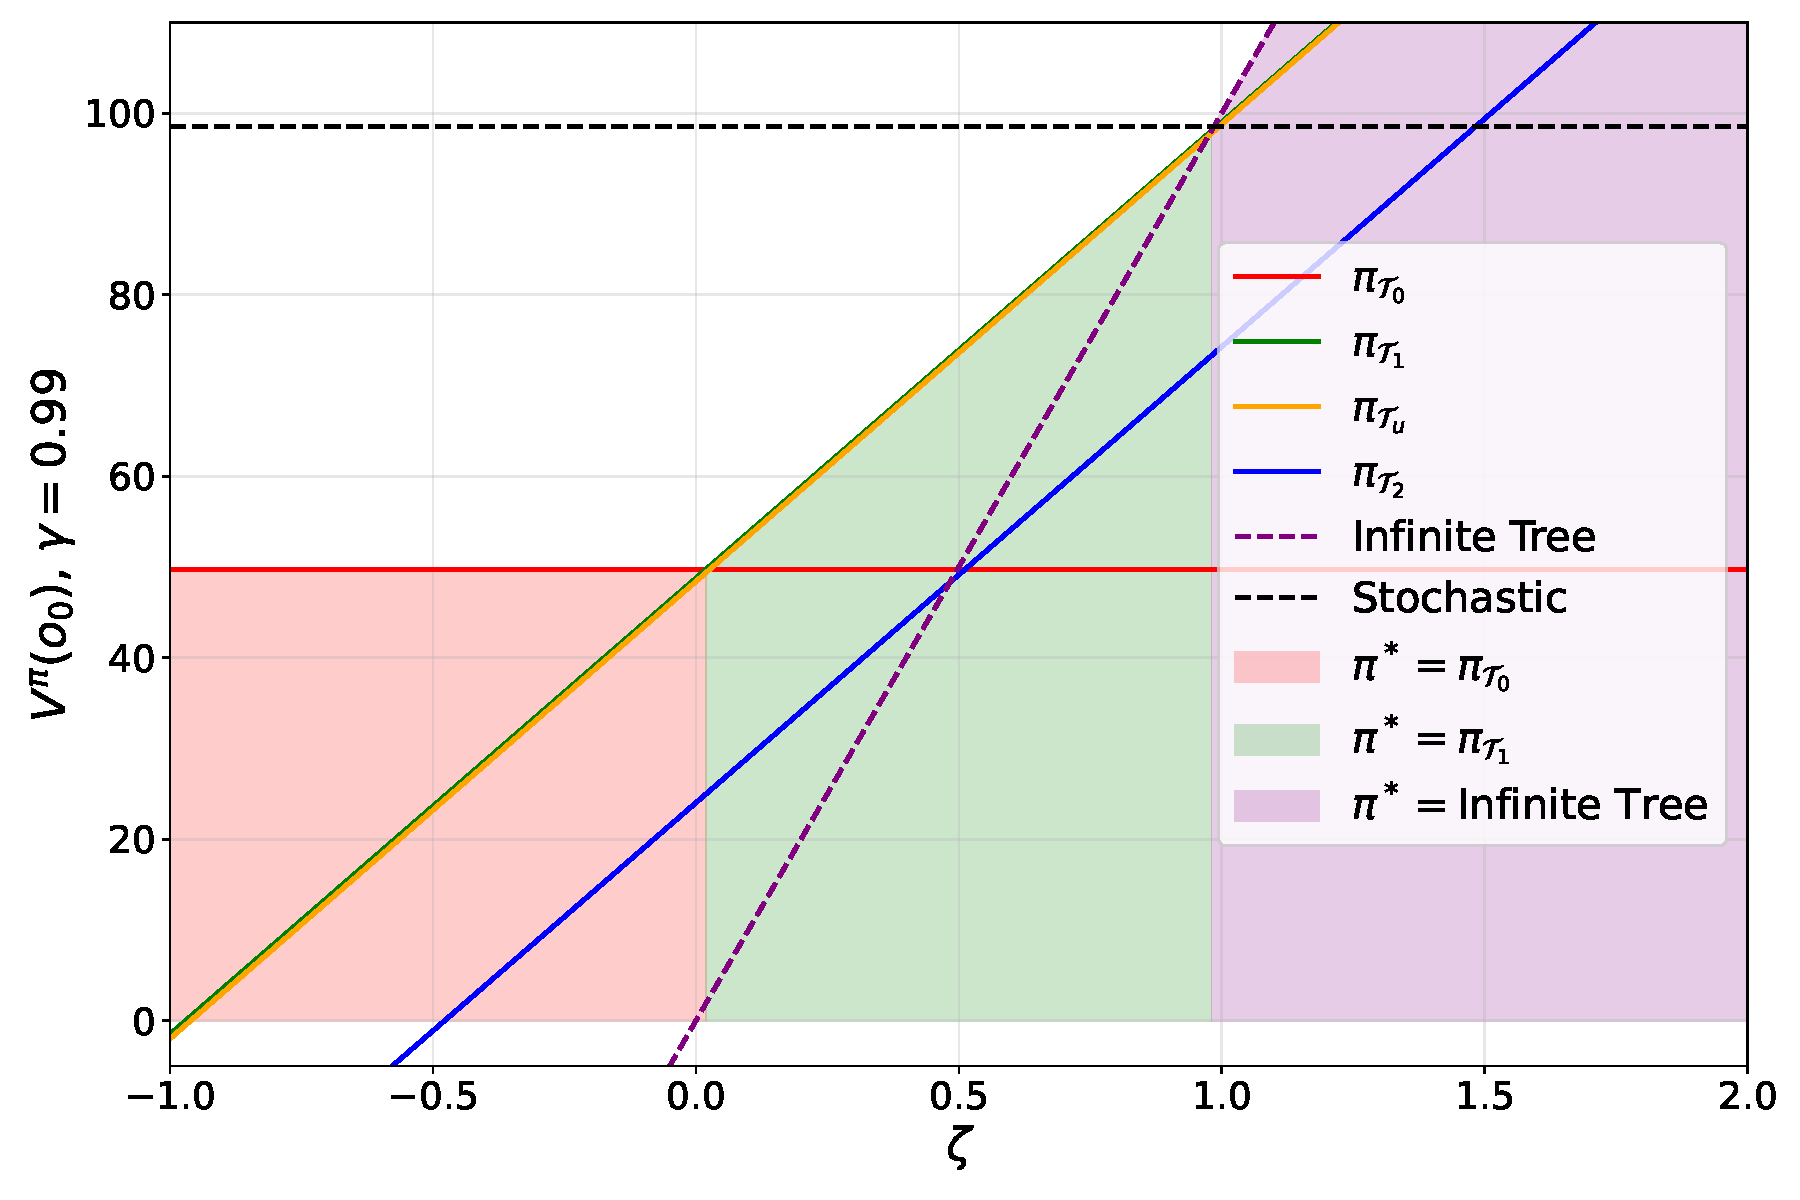
\includegraphics[width=0.6\textwidth]{images/images_part1/objective_values_plot.pdf}
        \caption{Interpretable RL objective values (\ref{def:irl}) of different partially observable policies as functions of $\zeta$. Shaded areas show the optimal \textit{deterministic} partially observable policies in different ranges of $\zeta$ values.}\label{fig:objectives}
    \end{figure}
\paragraph{Depth-0 decision tree:} has only one leaf node that takes a single base action indefinitely.
For this type of tree the best reward achievable is to take actions that maximize the probability of reaching the objective $\rightarrow$ or $\downarrow$. In that case the objective value of such tree is:
In the goal state $G = (1, 0)$, the value of the depth-0 tree $\mathcal{T}_0$ is:
\begin{align*}
    V^{\mathcal{T}_0}_G &= 1 + \gamma + \gamma^2 + \dots \\
    &= \overset{\infty}{\underset{t=0}\sum} \gamma^t \\
    &= \frac{1}{1 - \gamma}
\end{align*}
In the state $(0, 0)$ when the policy repeats going right respectively in the state $(0, 1)$ when the policy repeats going down, the value is:
\begin{align*}
    V^{\mathcal{T}_0}_{S_0} &= 0 + \gamma V^{\mathcal{T}_0}_g \\
    &= \gamma V^{\mathcal{T}_0}_G
\end{align*}
In the other states the policy never gets positive rewards; $V^{\mathcal{T}_0}_{S_1} = V^{\mathcal{T}_0}_{S_2} = 0$. Hence:
\begin{align*}
J(\mathcal{T}_0) &= \frac{1}{4} V^{\mathcal{T}_0}_G + \frac{1}{4} V^{\mathcal{T}_0}_{S_0}+ \frac{1}{4} V^{\mathcal{T}_0}_{S_1}+ \frac{1}{4} V^{\mathcal{T}_0}_{S_2} \\
&= \frac{1}{4} V^{\mathcal{T}_0}_G + \frac{1}{4} \gamma V^{\mathcal{T}_0}_G + 0 + 0\\
&= \frac{1}{4} \frac{1}{1 - \gamma} + \frac{1}{4} \gamma \frac{1}{1 - \gamma} \\
&= \frac{1 + \gamma}{4(1 - \gamma)}
\end{align*}

\paragraph{Unbalanced depth-2 decision tree:}the unbalanced depth-2 decision tree  takes an information gathering action $x\leq0.5$ then either takes the $\downarrow$ action or takes a second information $y\leq0.5$ followed by $\rightarrow$ or $\downarrow$.
In states $G$ and $S_2$, the value of the unbalanced tree is the same as for the depth-1 tree.
In states $S_0$ and $S_1$, the policy takes two information gathering actions before taking a base action and so on:
\begin{align*}
    V^{\mathcal{T}_{u}}_{S_0} &= \zeta + \gamma \zeta + \gamma ^ 2 0 + \gamma ^ 3 V^{\mathcal{T}_1}_G
\end{align*} 
\begin{align*}
    V^{\mathcal{T}_{u}}_{S_1} &= \zeta + \gamma \zeta + \gamma ^ 2 0 + \gamma ^ 3 V^{\mathcal{T}_u}_{S_0} \\ 
    &= \zeta + \gamma \zeta + \gamma ^ 2 0 + \gamma ^ 3 (\zeta + \gamma \zeta + \gamma ^ 2 0 + \gamma ^ 3 V^{\mathcal{T}_1}_G) \\
    &= \zeta + \gamma \zeta + \gamma ^ 3 \zeta + \gamma ^ 4 \zeta + \gamma ^ 6 V^{\mathcal{T}_1}_G
\end{align*}
We get:
\begin{align*}
    J(\mathcal{T}_{u}) &= \frac{1}{4} V^{\mathcal{T}_u}_G + \frac{1}{4} V^{\mathcal{T}_u}_{S_0} + \frac{1}{4}V^{\mathcal{T}_u}_{S_1} + \frac{1}{4}V^{\mathcal{T}_u}_{S_2} \\
    &=  \frac{1}{4} V^{\mathcal{T}_1}_G + \frac{1}{4}(\zeta + \gamma \zeta + \gamma ^ 3 V^{\mathcal{T}_1}_G) + \frac{1}{4} (\zeta + \gamma \zeta + \gamma ^ 3 \zeta + \gamma ^ 4 \zeta + \gamma ^ 6 V^{\mathcal{T}_1}_G) + \frac{1}{4}V^{\mathcal{T}_1}_{S_2} \\
    &= \frac{1}{4} (\frac{\zeta + \gamma}{1-\gamma^2}) + \frac{1}{4}(\frac{\gamma\zeta + \gamma^4 + \zeta -\gamma^2\zeta}{1-\gamma^2}) + \frac{1}{4} (\zeta + \gamma \zeta + \gamma ^ 3 \zeta + \gamma ^ 4 \zeta + \gamma ^ 6 V^{\mathcal{T}_1}_G) + \frac{1}{4}V^{\mathcal{T}_1}_{S_2} \\
    &= \frac{1}{4} (\frac{\zeta + \gamma}{1-\gamma^2}) + \frac{1}{4}(\frac{\gamma\zeta + \gamma^4 + \zeta -\gamma^2\zeta}{1-\gamma^2}) + \frac{1}{4} (\frac{\zeta + \gamma\zeta -\gamma^2\zeta-\gamma^5\zeta+\gamma^6\zeta+\gamma^7}{1-\gamma^2}) + \frac{1}{4}V^{\mathcal{T}_1}_{S_2} \\
    &= \frac{1}{4} (\frac{\zeta + \gamma}{1-\gamma^2}) + \frac{1}{4}(\frac{\gamma\zeta + \gamma^4 + \zeta -\gamma^2\zeta}{1-\gamma^2}) + \frac{1}{4} (\frac{\zeta + \gamma\zeta -\gamma^2\zeta-\gamma^5\zeta+\gamma^6\zeta+\gamma^7}{1-\gamma^2}) + \frac{1}{4}(\frac{\zeta + \gamma ^ 3}{1-\gamma^2}) \\
    &= \frac{\zeta(4+2\gamma-2\gamma^2-\gamma^5+\gamma^6)+\gamma+\gamma^3+\gamma^4+\gamma^7}{4(1-\gamma^2)}
\end{align*}
\paragraph{The balanced depth-2 decision tree:}alternates in every state between taking the two available information gathering actions and then a base action.
The value of the policy in the goal state is:
\begin{align*}
    V^{\mathcal{T}_2}_{G} &= \zeta + \gamma\zeta + \gamma^2 + \gamma^3\zeta + \gamma^4\zeta + \dots \\
    &= \overset{\infty}{\underset{t=0}\sum} \gamma^{3t}\zeta + \overset{\infty}{\underset{t=0}\sum} \gamma^{3t+1}\zeta + \overset{\infty}{\underset{t=0}\sum} \gamma^{3t+2} \\
    &= \frac{\zeta}{1-\gamma^3} + \frac{\gamma\zeta}{1-\gamma^3} + \frac{\gamma^2}{1-\gamma^3}
\end{align*}
Following the same reasoning for other states we find the objective value for the depth-2 decision tree policy to be:
\begin{align*}
    J(\mathcal{T}_2) &=\frac{1}{4} V^{\mathcal{T}_2}_G + \frac{2}{4} V^{\mathcal{T}_2}_{S_2} + \frac{1}{4} V^{\mathcal{T}_2}_{S_1} \\
    &= \frac{1}{4} V^{\mathcal{T}_2}_G + \frac{2}{4}(\zeta + \gamma\zeta + \gamma^2 0 + \gamma^3V^{\mathcal{T}_2}_G) + \frac{1}{4} (\zeta+\gamma\zeta+\gamma^2 0 + \gamma^3\zeta+\gamma^4\zeta+\gamma^5 0 +\gamma^6 V^{\mathcal{T}_2}_G) \\
    &= \frac{\zeta(3+3\gamma)+\gamma^2+\gamma^5+\gamma^8}{4(1-\gamma^3)}
\end{align*}
\paragraph{Infinite tree:} we also consider the infinite tree policy that repeats an information gathering action forever and has objective: $J(\mathcal{T_{\text{inf}}}) = \frac{\zeta}{1-\gamma}$

\paragraph{Stochastic policy:} the other non-trivial policy that can be learned by solving a partially observable IBMDP is the stochastic policy that guarantees to reach $G$ after some time: fifty percent chance to do $\rightarrow$ and fifty percent chance to do $\downarrow$.
This stochastic policy has objective value:
\begin{align*}
    V^{\text{stoch}}_G &= \frac{1}{1-\gamma} \\
    V^{\text{stoch}}_{S_0} &= 0 + \frac{1}{2}\gamma V^{\text{stoch}}_G + \frac{1}{2}\gamma V^{\text{stoch}}_{S_1} \\
    V^{\text{stoch}}_{S_2} &= 0 + \frac{1}{2}\gamma V^{\text{stoch}}_G + \frac{1}{2}\gamma V^{\text{stoch}}_{S_1} = V^{\text{stoch}}_{S_0} \\
    V^{\text{stoch}}_{S_1} &= 0 + \frac{1}{2}\gamma V^{\text{stoch}}_{S_2} + \frac{1}{2}\gamma V^{\text{stoch}}_G = \frac{1}{2}\gamma V^{\text{stoch}}_{S_0} + \frac{1}{2}\gamma V^{\text{stoch}}_G
\end{align*}
Solving these equations:
\begin{align*}
    V^{\text{stoch}}_{S_1} &= \frac{1}{2}\gamma V^{\text{stoch}}_{S_0} + \frac{1}{2}\gamma V^{\text{stoch}}_G \\
    &= \frac{1}{2}\gamma (\frac{1}{2}\gamma V^{\text{stoch}}_G + \frac{1}{2}\gamma V^{\text{stoch}}_{S_1}) + \frac{1}{2}\gamma V^{\text{stoch}}_G \\
    &= \frac{1}{4}\gamma^2 V^{\text{stoch}}_G + \frac{1}{4}\gamma^2 V^{\text{stoch}}_{S_1} + \frac{1}{2}\gamma V^{\text{stoch}}_G \\
    V^{\text{stoch}}_{S_1} - \frac{1}{4}\gamma^2 V^{\text{stoch}}_{S_1} &= \frac{1}{4}\gamma^2 V^{\text{stoch}}_G + \frac{1}{2}\gamma V^{\text{stoch}}_G \\
    V^{\text{stoch}}_{S_1}(1 - \frac{1}{4}\gamma^2) &= (\frac{1}{4}\gamma^2 + \frac{1}{2}\gamma) V^{\text{stoch}}_G \\
    V^{\text{stoch}}_{S_1} &= \frac{\frac{1}{4}\gamma^2 + \frac{1}{2}\gamma}{1 - \frac{1}{4}\gamma^2} V^{\text{stoch}}_G \\
    &= \frac{\gamma(\frac{1}{4}\gamma + \frac{1}{2})}{1 - \frac{1}{4}\gamma^2} \cdot \frac{1}{1-\gamma} \\
    &= \frac{\gamma(\frac{1}{4}\gamma + \frac{1}{2})}{(1 - \frac{1}{4}\gamma^2)(1-\gamma)}
\end{align*}
\begin{align*}
    V^{\text{stoch}}_{S_0} &= \frac{1}{2}\gamma V^{\text{stoch}}_G + \frac{1}{2}\gamma V^{\text{stoch}}_{S_1} \\
    &= \frac{1}{2}\gamma \cdot \frac{1}{1-\gamma} + \frac{1}{2}\gamma \cdot \frac{\gamma(\frac{1}{4}\gamma + \frac{1}{2})}{(1 - \frac{1}{4}\gamma^2)(1-\gamma)} \\
    &= \frac{\frac{1}{2}\gamma}{1-\gamma} + \frac{\frac{1}{2}\gamma^2(\frac{1}{4}\gamma + \frac{1}{2})}{(1 - \frac{1}{4}\gamma^2)(1-\gamma)} \\
    &= \frac{\frac{1}{2}\gamma(1 - \frac{1}{4}\gamma^2) + \frac{1}{2}\gamma^2(\frac{1}{4}\gamma + \frac{1}{2})}{(1 - \frac{1}{4}\gamma^2)(1-\gamma)} \\
    &= \frac{\frac{1}{2}\gamma - \frac{1}{8}\gamma^3 + \frac{1}{8}\gamma^3 + \frac{1}{4}\gamma^2}{(1 - \frac{1}{4}\gamma^2)(1-\gamma)} \\
    &= \frac{\frac{1}{2}\gamma + \frac{1}{4}\gamma^2}{(1 - \frac{1}{4}\gamma^2)(1-\gamma)} \\
    &= \frac{\gamma(\frac{1}{2} + \frac{1}{4}\gamma)}{(1 - \frac{1}{4}\gamma^2)(1-\gamma)}
\end{align*}
\begin{align*}
    J(\mathcal{T}_{\text{stoch}}) &= \frac{1}{4}(V^{\text{stoch}}_G + V^{\text{stoch}}_{S_0} + V^{\text{stoch}}_{S_1} + V^{\text{stoch}}_{S_2}) \\
    &= \frac{1}{4}\left(\frac{1}{1-\gamma} + 2 \cdot \frac{\gamma(\frac{1}{2} + \frac{1}{4}\gamma)}{(1 - \frac{1}{4}\gamma^2)(1-\gamma)} + \frac{\gamma(\frac{1}{4}\gamma + \frac{1}{2})}{(1 - \frac{1}{4}\gamma^2)(1-\gamma)}\right) \\
    &= \frac{1}{4}\left(\frac{1}{1-\gamma} + \frac{2\gamma(\frac{1}{2} + \frac{1}{4}\gamma) + \gamma(\frac{1}{4}\gamma + \frac{1}{2})}{(1 - \frac{1}{4}\gamma^2)(1-\gamma)}\right) \\
    &= \frac{1}{4}\left(\frac{1}{1-\gamma} + \frac{\gamma + \frac{1}{2}\gamma^2 + \frac{1}{4}\gamma^2 + \frac{1}{2}\gamma}{(1 - \frac{1}{4}\gamma^2)(1-\gamma)}\right) \\
    &= \frac{1}{4}\left(\frac{1}{1-\gamma} + \frac{\frac{3}{2}\gamma + \frac{3}{4}\gamma^2}{(1 - \frac{1}{4}\gamma^2)(1-\gamma)}\right) \\
    &= \frac{1}{4}\left(\frac{1 - \frac{1}{4}\gamma^2 + \frac{3}{2}\gamma + \frac{3}{4}\gamma^2}{(1 - \frac{1}{4}\gamma^2)(1-\gamma)}\right) \\
    &= \frac{1}{4}\left(\frac{1 + \frac{3}{2}\gamma + \frac{1}{2}\gamma^2}{(1 - \frac{1}{4}\gamma^2)(1-\gamma)}\right) \\
    &= \frac{1 + \frac{3}{2}\gamma + \frac{1}{2}\gamma^2}{4(1 - \frac{1}{4}\gamma^2)(1-\gamma)}
\end{align*}

\section{Hyperparameters}\label{sec:hp-pomdp}
\begin{table}
\small
\centering
\caption{PG Hyperparameter Space (140 combinations)}
\begin{tabular}{lll}
\toprule
\textbf{Hyperparameter} & \textbf{Values} & \textbf{Description} \\
\midrule
Learning Rate (lr) & 0.001, 0.005, 0.01, 0.05, 0.1 & Policy gradient step size \\
Entropy Regularization (tau) & -1.0, -0.1, -0.01, 0.0, 0.01, 0.1, 1.0 & Entropy regularization coefficient \\
Temperature (eps) & 0.01, 0.1, 1.0, 10 & Softmax temperature \\
Episodes per Update (n\_steps) & 20, 200, 2000 & Number of episodes per policy update \\
\bottomrule
\end{tabular}
\end{table}

\begin{table}
\small
\centering
\caption{PG-IBMDP Hyperparameter Space (140 combinations)}
\begin{tabular}{lll}
\toprule
\textbf{Hyperparameter} & \textbf{Values} & \textbf{Description} \\
\midrule
Learning Rate (lr) & 0.001, 0.005, 0.01, 0.05, 0.1 & Policy gradient step size \\
Entropy Regularization (tau) & -1.0, -0.1, -0.01, 0.0, 0.01, 0.1, 1.0 & Entropy regularization coefficient \\
Temperature (eps) & 0.01, 0.1, 1.0, 10 & Softmax temperature \\
Episodes per Update (n\_steps) & 10, 100, 1000 & Number of episodes per policy update \\
\bottomrule
\end{tabular}
\end{table}


\begin{table}
\small
\centering
\caption{QL Hyperparameter Space (192 combinations)}
\begin{tabular}{lll}
\toprule
\textbf{Hyperparameter} & \textbf{Values} & \textbf{Description} \\
\midrule
Epsilon Schedules & (0.3, 1), (0.3, 0.99), (1, 1) & Initial exploration and decrease rate \\
Epsilon Schedules & (0.1, 1), (0.1, 0.99), (0.3, 0.99) & Initial exploration and decrease rate \\
Lambda & 0.0, 0.3, 0.6, 0.9 & Eligibility trace decay \\
Learning Rate (lr\_o) & 0.001, 0.005, 0.01, 0.1 & Observation Q-learning rate \\
Optimistic & True, False & Optimistic initialization \\
\bottomrule
\end{tabular}
\end{table}

\begin{table}
\small
\centering
\caption{QL-Asym Hyperparameter Space (768 combinations)}
\begin{tabular}{lll}
\toprule
\textbf{Hyperparameter} & \textbf{Values} & \textbf{Description} \\
\midrule
Epsilon Schedules & (0.3, 1), (0.3, 0.99), (1, 1) & Initial exploration and decrease rate \\
Epsilon Schedules & (0.1, 1), (0.1, 0.99), (0.3, 0.99) & Initial exploration and decrease rate \\
Lambda & 0.0, 0.3, 0.6, 0.9 & Eligibility trace decay \\
Learning Rate (lr\_o) & 0.001, 0.005, 0.01, 0.1 & Observation Q-learning rate \\
Learning Rate (lr\_v) & 0.001, 0.005, 0.01, 0.1 & State-action Q-learning rate \\
Optimistic & True, False & Optimistic initialization \\
\bottomrule
\end{tabular}
\end{table}

\begin{table}
\small
\centering
\caption{QL-IBMDP Hyperparameter Space (192 combinations)}
\begin{tabular}{lll}
\toprule
\textbf{Hyperparameter} & \textbf{Values} & \textbf{Description} \\
\midrule
Epsilon Schedules & (0.3, 1), (0.3, 0.99), (1, 1) & Initial exploration and decrease rate \\
Epsilon Schedules & (0.1, 1), (0.1, 0.99), (0.3, 0.99) & Initial exploration and decrease rate \\
Lambda & 0.0, 0.3, 0.6, 0.9 & Eligibility trace decay \\
Learning Rate (lr\_v) & 0.001, 0.005, 0.01, 00.1 & State-action Q-learning rate \\
Optimistic & True, False & Optimistic initialization \\
\bottomrule
\end{tabular}
\end{table}

\begin{table}
\small
\centering
\caption{SARSA Hyperparameter Space (192 combinations)}
\begin{tabular}{lll}
\toprule
\textbf{Hyperparameter} & \textbf{Values} & \textbf{Description} \\
\midrule
Epsilon Schedules & (0.3, 1), (0.3, 0.99), (1, 1) & Initial exploration and decrease rate \\
Epsilon Schedules & (0.1, 1), (0.1, 0.99), (0.3, 0.99) & Initial exploration and decrease rate \\
Lambda & 0.0, 0.3, 0.6, 0.9 & Eligibility trace decay \\
Learning Rate (lr\_o) & 0.001, 0.005, 0.01, 0.1 & Observation SARSA learning rate \\
Optimistic & True, False & Optimistic initialization \\
\bottomrule
\end{tabular}
\end{table}

\begin{table}
\small
\centering
\caption{SARSA-Asym Hyperparameter Space (768 combinations)}
\begin{tabular}{lll}
\toprule
\textbf{Hyperparameter} & \textbf{Values} & \textbf{Description} \\
\midrule
Epsilon Schedules & (0.3, 1), (0.3, 0.99), (1, 1) & Initial exploration and decrease rate \\
Epsilon Schedules & (0.1, 1), (0.1, 0.99), (0.3, 0.99) & Initial exploration and decrease rate \\
Lambda & 0.0, 0.3, 0.6, 0.9 & Eligibility trace decay \\
Learning Rate (lr\_o) & 0.001, 0.005, 0.01, 0.1 & Observation SARSA learning rate \\
Learning Rate (lr\_v) & 0.001, 0.005, 0.01, 0.1 & State-action SARSA learning rate \\
Optimistic & True, False & Optimistic initialization \\
\bottomrule
\end{tabular}
\end{table}

\begin{table}
\small
\centering
\caption{SARSA-IBMDP Hyperparameter Space (192 combinations)}
\begin{tabular}{lll}
\toprule
\textbf{Hyperparameter} & \textbf{Values} & \textbf{Description} \\
\midrule
Epsilon Schedules & (0.3, 1), (0.3, 0.99), (1, 1) & Initial exploration and decrease rate \\
Epsilon Schedules & (0.1, 1), (0.1, 0.99), (0.3, 0.99) & Initial exploration and decrease rate \\
Lambda & 0.0, 0.3, 0.6, 0.9 & Eligibility trace decay \\
Learning Rate (lr\_v) & 0.001, 0.005, 0.01, 0.1 & State-action SARSA learning rate \\
Optimistic & True, False & Optimistic initialization \\
\bottomrule
\end{tabular}
\end{table}


\begin{table}
    \centering
    \begin{tabular}{|l|c|c|c|}
    \textbf{Hyperparameter} & \textbf{Asym Q-learning (10/10)} & \textbf{Asym Sarsa (10/10)} & \textbf{PG (4/10)} \\
    \toprule
    epsilon\_start & 1.0 & 1.0 & - \\
    epsilon\_decay & 0.99 & 0.99 & - \\
    batch\_size & 1 & 1 & - \\
    lambda\_ & 0.0 & 0.0 & - \\
    lr\_o & 0.01 & 0.1 & - \\
    lr\_v & 0.1 & 0.005 & - \\
    optimistic & False & False & - \\
    lr & - & - & 0.05 \\
    tau & - & - & 0.1 \\
    eps & - & - & 0.1 \\
    n\_steps & - & - & 2000 \\
    \bottomrule
    \end{tabular}
    \caption{Best hyperparameters for each algorithm on the POIBMDP problem}
    \label{tab:algorithm-hyperparameters}
    \end{table}
